\documentclass[%11pt,
  use style = classical,
  % numbered answer,
  % numbered question,
  scroll,
]{Q-and-A}

\def\PackageVersion{2023/11/11}
\def\PackageSubVersion{}

\newcommand{\QApackage}{{\normalfont\textsf{Q-and-A}}}


\title{\QApackage{}\\\smallskip\itshape Typesetting Q\&A-style conversation made easier}
\author{Jinwen XU}
% \thanks{Corresponding to: \texttt{\QApackage{}~\PackageVersion\PackageSubVersion}}
\date{\TheDate{\PackageVersion}[only-year-month], in Paris}


\newcommand{\meta}[1]{$\langle${\normalfont\itshape#1}$\rangle$}


\begin{document}

\maketitle

"
  Corresponding to: {\normalfont\texttt{\QApackage{}~\PackageVersion\PackageSubVersion}}.


##+ {Introduction}

?
  What is this?

:
  \QApackage{} is a \LaTeX{} document class for you to typeset Q\&A-style conversation. It turns a simple pure text Q\&A dialog like this:

  == {code/Q-and-A-doc-code-sample-content.tex}

  into a carefully designed document like this:

  \begin{center}
    \fbox{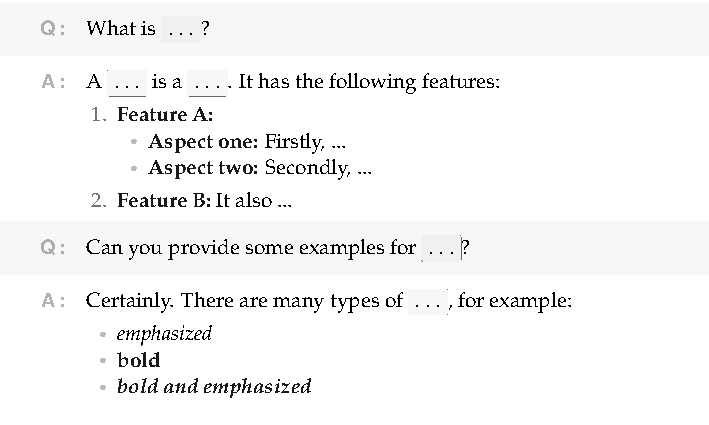
\includegraphics[width=.67\textwidth]{code/Q-and-A-doc-code-sample-content-result.pdf}}
  \end{center}


##+ {Preparation}

?
  That is nice. How can I use it? Is there anything that needs to be prepared?

:
  You should make sure that this document class is properly installed.

  If you are using TeX Live 2024 or newer, or the most recent version of MikTeX, then this package should already be included, and you don't need to do anything.

  Otherwise, you need to check for package update to see if you can receive it. In case not, you can always go to \href{https://ctan.org/pkg/Q-and-A}{the CTAN page} to download the `.zip` file with all related files included.


##+ {Usage}

?
  Now that I have successfully installed it, could you propose an example of usage?

:
  Of course. A typical document looks like this:

  == [latex] {code/Q-and-A-doc-code-sample-document.tex}

  The available class options include:
  \begin{itemize}
    \item Font size options such as `11pt`, `12pt`.
    \item `scroll`: turn the scroll mode on, which generates a single-page pdf similar to a long screenshot. It is recommended to use this option if your document contains some large piece of code.
    \item `use theme = \meta{theme}`: use the selected theme, available choices include: `default` (like the current document), `ChatGPT-light` and `ChatGPT-dark` (see the demo documents).
    \item `numbered question`, or `question number`: enable the numbering of questions.
    \item `numbered answer`, or `answer number`: enable the numbering of answers.
    \item `answer outside the box`, or `answer out of the box` (or even omit `the`): enable another implementation for printing the answer that does not involve putting it into a colored box. This would be useful if the answers contain many long pieces of code while you still want the pages to break normally.
  \end{itemize}

?
  What about the main content?

:
  You have already seen an example of the main content. As you might have noticed, there are several syntaxes. Let me explain.

  [Questions (Q), Answers (A), and Narrations (N)]
  \begin{itemize}
    \item A question begins with the prefix `Q:` or `?`.
    \item An answer begins with the prefix `A:` or `:`.
    \item A narration begins with the prefix `N:` or `"`.
  \end{itemize}
  >>> Note that this depends on the current language. The prefixes `?`, `:` and `"` being universal, yet~—
  \begin{itemize}
    \item for French, it is Q\&R\&N, thus the alphabetical prefixes become `Q:`, `R:` and `N:`;
    \item for German, it is F\&A\&E, thus the alphabetical prefixes become `F:`, `A:` and `E:`;
    \item for Italian, it is D\&R\&N, thus the alphabetical prefixes become `D:`, `R:` and `N:`;
    \item for Portuguese and Brazilian, it is P\&R\&N, thus the alphabetical prefixes become `P:`, `R:` and `N:`;
    \item for Russian, it is B\&O\&P, thus the alphabetical prefixes become `B:`, `O:` and `P:`;
    \item for Spanish, it is P\&R\&N, thus the alphabetical prefixes become `P:`, `R:` and `N:`;
    \item for simplified Chinese, it is also possible to use the prefix `问:` for questions, `答:` for answers, and `注:` for narrations; similarly for traditional Chinese;
    \item for Chinese or Japanese, it is also possible to use the prefix `?` for questions, `:` for answers, and `“`, `”` or `「` for narrations.
  \end{itemize}

  [Emphasize and Bold]
  \begin{itemize}
    \item Use `\textasterisk\meta{text}\textasterisk` to emphasis `\meta{text}`.
    \item Use `\textasterisk\textasterisk\meta{text}\textasterisk\textasterisk` to make `\meta{text}` into boldface.
    \item Use `\textasterisk\textasterisk\textasterisk\meta{text}\textasterisk\textasterisk\textasterisk` to combine the previous effects.
  \end{itemize}

  [Enumerate and Itemize]
    \begin{itemize}
      \item **Emphasized version:**
      \begin{itemize}
        \item An emphasized `enumerate` is marked by `[\meta{text}]` *at the beginning*, where `\meta{text}` is the text to be emphasized. The numbering is reset at the end of each answer.
        \QANote{If you wish to restart the numbering from \( 1 \), write an asterisk after the final bracket: `[\meta{text}]\textasterisk`.}
        \item An emphasized `itemize` is marked by `[\textasterisk\meta{text}]`, where `\meta{text}` is the text to be emphasized.
      \end{itemize}
      \item **Normal version:**
      \begin{itemize}
        \item When `\meta{text}` is empty, you get the usual appearance of `enumerate` or `itemize`.
      \end{itemize}
    \end{itemize}
    \QANote{With this method of writing, each emphasized `enumerate` and `itemize` must be put into a separate paragraph, and the lists cannot be nested. The usual `enumerate` and `itemize` environments would still be useful if you need nested lists.}

  [Images]
  Displayed images can be included via one of the following ways:
  \begin{itemize}
    \item `\textvert\textvert{} <\meta{width}> \{\meta{image file name}\}` or `\textvert\textvert{} \{\meta{image file name}\} <\meta{width}>`: display in the center.
    \item `\textleftparen\textleftparen{} <\meta{width}> \{\meta{image file name}\}` or `\textleftparen\textleftparen{} \{\meta{image file name}\} <\meta{width}>`: display on the left.
    \item `\textrightparen\textrightparen{} <\meta{width}> \{\meta{image file name}\}` or `\textrightparen\textrightparen{} \{\meta{image file name}\} <\meta{width}>`: display on the right.
  \end{itemize}
  \QANote{The `\meta{width}` is optional. Here, `\meta{width}` is a number like `0.75`, the unit is `\textbackslash linewidth`. When `\meta{width}` is not given, the width would be full `\textbackslash linewidth`.}
  \begin{itemize}
    \item For centered image, the caption can be written via `\textgreater\textgreater{} \meta{caption text}`.
  \end{itemize}
  % \QANote{Currently, the `\meta{caption text}` shall be directly printed in the center. You may wish to add a pair of parentheses around it.}

  [Code]
  Due to the current implementation of this document class, it is unfortunate that you cannot directly insert source code in your document. There are some workarounds, though.
  \begin{itemize}
    \item For *inline* code, you may simply write it between two backticks `\textbacktick\meta{code}\textbacktick`, similar to the Markdown syntax. However, be aware that special characters need to be escaped, for example, `\textbackslash` should be written as `\textbackslash textbackslash`, `\{` should be written as `\textbackslash\{`, `\%` should be written as `\textbackslash\%`, etc.
    \item For *displayed* code, store the code into a separate file, and then use `\textequalsign\textequalsign{} \{\meta{file name}\}` to print~it. You may also use an optional argument like `\textequalsign\textequalsign{} [\meta{language}] \{\meta{file name}\}` to select the language of your code.
    \QANote{If the answers contain many long pieces of code, you may consider using the class option `answer outside the box`.}
  \end{itemize}

  [Sections]
  \begin{itemize}
    \item You may start a new (*unnumbered*) ---
    \begin{itemize}
      \item section, via `\textsharp\textsharp{} \{\meta{section title}\}`;
      \item subsection, via `\textsharp\textsharp\textsharp{} \{\meta{subsection title}\}`;
      \item subsubsection, via `\textsharp\textsharp\textsharp\textsharp{} \{\meta{subsubsection title}\}`;
    \end{itemize}
    \item If you wish to use the *numbered* version, write `\textsharp\textsharp+`, `\textsharp\textsharp\textsharp+` and `\textsharp\textsharp\textsharp\textsharp+` instead.
  \end{itemize}

  [Input/Include Files]
  \begin{itemize}
    \item Use `\textcolon\textcolon{} \{\meta{file name}\}` to input a file.
    \item Use `\textcolon\textcolon\textcolon{} \{\meta{file name}\}` to include a file.
  \end{itemize}

  \medskip

  And don't forget that you are still using \LaTeX, so images, tables and lists can be written as usual.

  \medskip

  >>> Currently, the default style for showing tables has not been settled (since the color configuration for tables with or without headers would be slightly different). As a temporary solution, it is recommended for you to consult the several nice answers of this question: \url{https://tex.stackexchange.com/q/10224}.


##+ {Cautions}

?
  I see. Is there anything else for me to be careful about?

:
  Glad that you asked. Here are several things that should be taken care of:
  \begin{itemize}
    \item A question, answer or narration should always begin in a new paragraph.
    \item An emphasized `enumerate` should also begin in a new paragraph. An emphasized `itemize` should usually begin in a new paragraph, with the exception that it can (partially) be used within an `enumerate`.
    \item Likewise, a `section`/`subsection`/`subsubsection` should be placed in a separate paragraph.
    \item Input or inclusion of files should also be operated in a separate paragraph.
    \item For emphasizing and bolding the text, it would be necessary to separate the asterisks with~`\{\}` in some special cases: `\textasterisk\textasterisk like\textasterisk\textasterisk\{\}\textasterisk\textasterisk\textasterisk this\textasterisk\textasterisk\textasterisk\{\}\textasterisk one\textasterisk`.
    \item Due to the recognition of the syntax, you cannot directly use characters like `\textasterisk` as usual, especially in math mode. You should consider using an alternative macro, such as `\textbackslash ast` for `\textasterisk` in math mode, or define a command version of the character in the preamble, such as `\textbackslash textasterisk` for `\textasterisk`. A list of predefined commands are:
    \begin{itemize}
      \item `\textbackslash textasterisk` for `\textasterisk`;
      \item `\textbackslash textbacktick` for `\textbacktick`;
      \item `\textbackslash textcolon` for `\textcolon`;
      \item `\textbackslash textequalsign` for `\textequalsign`;
      \item `\textbackslash textleftparen` for `\textleftparen`;
      \item `\textbackslash textrightparen` for `\textrightparen`;
      \item `\textbackslash textsharp` for `\textsharp`.
      \item `\textbackslash textvert` for `\textvert`.
    \end{itemize}
    There are also a few that already provided by \LaTeX, such as:
    \begin{itemize}
      \item `\textbackslash textbackslash` for `\textbackslash`;
      \item `\textbackslash textgreater` for `\textgreater`;
      \item `\textbackslash textless` for `\textless`.
    \end{itemize}
  \end{itemize}


##+ {Customization}

?
  Now that we have learned the basic usage, I would like to know more. Can I customize the interface to suit my preferences, for instance?

:
  Certainly. Apart from using themes via class option, you may also change the identifiers and the labels for each role in the conversation.

  [Changing itentifiers]
  Instead of the default identifiers, such as `?` for questions, you may also use your preferred one. This can be done via the use of `\textbackslash QASetTypePrefix` in the preamble of your document.
  \begin{itemize}
    \item Use `\textbackslash QASetTypePrefix\{Q\}\{\meta{identifiers}\}` to set the identifiers for questions.
    \item Use `\textbackslash QASetTypePrefix\{A\}\{\meta{identifiers}\}` to set the identifiers for answers.
    \item Use `\textbackslash QASetTypePrefix\{N\}\{\meta{identifiers}\}` to set the identifiers for narrations.
  \end{itemize}
  Here, \meta{identifier} is a comma list of your specified identifiers. For example, the default identifier for narrations is preset via `\textbackslash QASetTypePrefix\{N\}\{N:,",“,”,「\}`.
  \QANote{Note that, due to its implementation, the identifier cannot contain comma `,` in it. If you wish to use an identifier that contains a comma, you may use `\textbackslash QAAddTypePrefix` instead, which only adds *one* identifier per use.}
  \QANote{Note also that, the identifiers are *reset* upon changing of language. Thus, you need to put your setting into the corresponding language configuration, for example, via `\textbackslash AddLanguageSetting[\meta{language name}]\{\meta{settings}\}`}

  [Changing labels]
  You may also change the labels. For example, from the text \textquote{Q:} to a logo icon. This can be done via the use of `\textbackslash SetLogoCode` in the preamble of your document.
  \begin{itemize}
    \item Use `\textbackslash SetLogoCode\{Q\}\{\meta{logo code}\}` to set the labels for questions.
    \item Use `\textbackslash SetLogoCode\{A\}\{\meta{logo code}\}` to set the labels for answers.
  \end{itemize}
  Here, \meta{logo code} is the actual code for displaying the corresponding label. For example, the default label for (unnumbered) questions is preset via `\textbackslash SetLogoCode\{Q\}\{\textbackslash textbf\{Q\textbackslash,:\}\}`.
  \QANote{In the demo document, you can find an example on how to use this command to specify a logo for each role in the conversation.}
  If you wish to include the question number or answer number, you may use the command `\textbackslash QAShowCounter`:
  \begin{itemize}
    \item Use `\textbackslash QAShowCounter\{Q\}` to step the counter of question and print it.
    \item Use `\textbackslash QAShowCounter\{A\}`  to step the counter of answer and print it.
  \end{itemize}
  For example, the default label for numbered questions is preset by adding `\textbackslash QAShowCounter\{Q\}` to the unnumbered version: `\textbackslash SetLogoCode\{Q\}\{\textbackslash textbf\{Q\textbackslash QAShowCounter\{Q\}\textbackslash,:\}\}`.


##+ {Known Issues}

?
  Is there any known issue with this document class?

:
  Unfortunately, yes `:(`.

  Below is a list of known issues:

  \begin{itemize}
    \item Currently, the code highlight is done by the package `listings`. Due to its own limitations, the result is still far from satisfactory. Using `minted` instead could improve the situation, but this would require `-shell-escape` and some external tweaking, thus it would still take some effort to make it work with the current document class.
    \item Due to the current implementation, one cannot direct write code (either inline or displayed) within the text (alternative solution has been proposed above).
    \item Due to the current implementation, when displaying the code, one may not be able to write some of the language name like `C\#` directly, but has to write an alternative name such as `csharp`.
    \item Due to the current implementation, one may not be able to directly write certain characters (such as `\textasterisk`) in the text, this might be especially inconvenient in math mode (temporary alternative solution has been proposed above).
    \item Due to the current implementation, the method for inputting and including subfiles doesn't really work like `\textbackslash input` and `\textbackslash include`. In particular, the current type of conversation would be reset, this might cause some confusion in certain cases.
    % \item The code block containing long piece of code usually won't properly break across the page (which is essentially why this documentation and the demo documents enabled the `scroll` mode).
    %% 2023-11-05, solved with the new option "answer outside the box".
    \item Due to the current implementation, though it is already possible to automatically adopt the identifiers and labels for supported languages, you still need to use the identifiers `Q`, `A` and `N` when setting them.
    \item Currently, for typesetting questions and answers, the text is in fact being put into some sort of `description` list (upon reflection, why did I do this? I could have simply put the label into margin...). As a result, the level of lists might be slightly messed up, which could sometimes lead to issues with the list labels.
  \end{itemize}


##+ {Getting Support}

?
  What should I do if I encounter any problem?

:
  If you run into any issues or have ideas for improvement, feel free to discuss on:
  \begin{center}
      \url{https://github.com/Jinwen-XU/Q-and-A/issues}
  \end{center}
  or email me via \href{mailto:ProjLib@outlook.com}{\texttt{ProjLib@outlook.com}}.


\vspace{3\baselineskip}

% ---

% "
%   Below is the code of the current document.

%   == [latex] {\jobname.tex}

\end{document}
